\chapter{The Effects of Linked Selection.}

\newthought{Genetic drift is not the only source of randomness} in the dynamics of
alleles. Alleles also experience random fluctuations in frequency due to
the fact that they present on a set of random genetic backgrounds with
different fitnesses. For example, when a beneficial allele arises via a single mutation, it arises on
a particular genetic background, i.e. a particular haplotype (Figure \ref{fig:HIV_sweep}A). Imagine this mutation arising in a region with no recombination, or in an
organism where genetic exchange is rare. If our beneficial allele
becomes established in the population, i.e. escapes loss by genetic
drift in those first few generations, it will start to increase in
frequency rapidly. As it rises in frequency, so will the alleles that happened to
be present on the haplotype that the mutation arose on (if those
other alleles are neutral or at least not too deleterious). These
other alleles are getting to 'hitchhiking' along. The alleles that are
not on that particular background are swept out of the population, so the net effect
of this selective sweep is to remove genetic diversity from the
population. Diversity will eventually recover, as new mutations
arise and some slowly drift up in frequency. But in the
short-term, selective sweeps remove genetic variation from
populations. 

\begin{figure}
\begin{center}
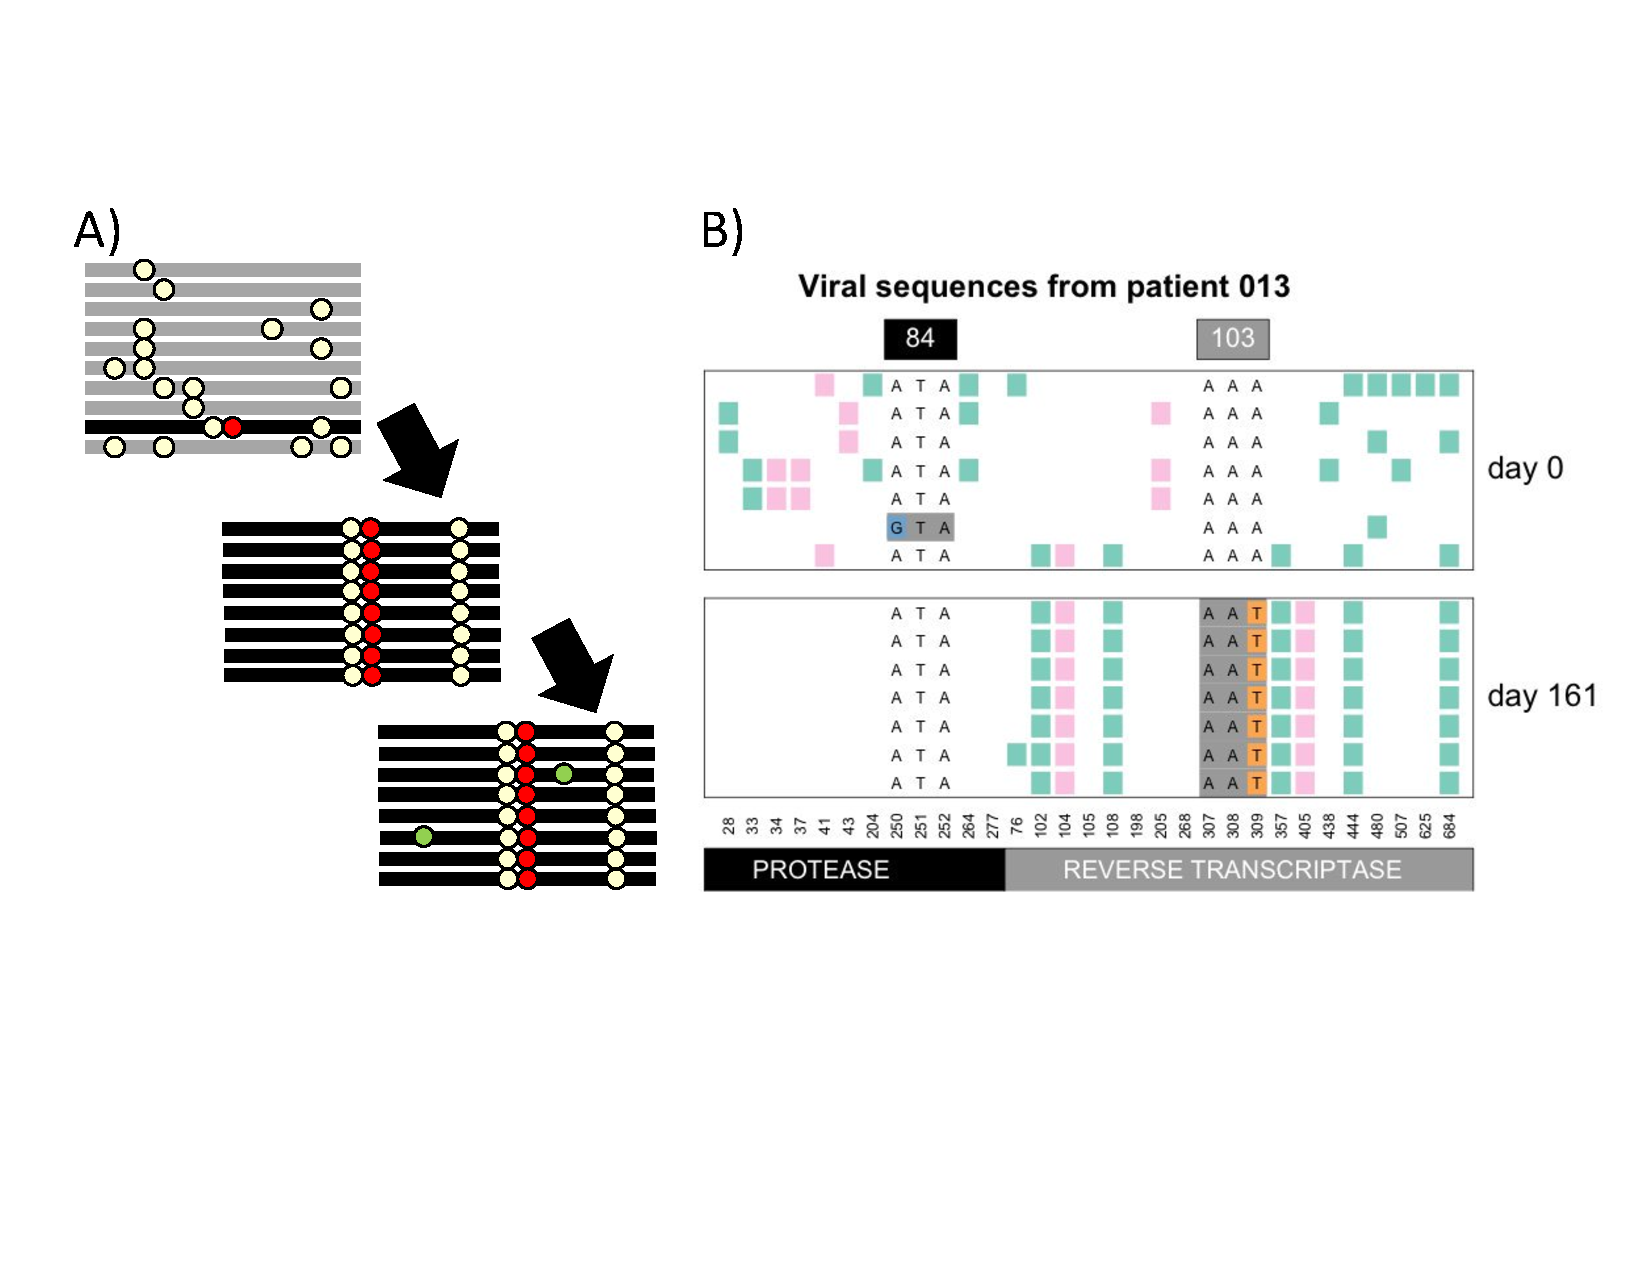
\includegraphics[width= \textwidth]{Journal_figs/recom_selection/Pleuni_HIV_sweep/HIV_no_recom_sweep.pdf}
\end{center}
\caption{{\bf A)} In the top panel, a selected mutation (red dot) arises
on a particular haplotype in the population. It sweeps to fixation,
carrying with it the haplotype on which it arose, middle panel,
erasing the standing genetic diversity in the region. The bottom panel
is some time after the selective sweep when some new neutral alleles (green
dots) have started to drift up in frequency. {\bf B)}  Top panel: HIV
sequences from a patient at the start of drug treatment in the
protease and retrotransposase coding regions. Bottom panel: A sample
161 days later, after a drug resistant mutation has spread, the A
$\rightarrow$ T in the $103^{rd}$ codon of retrotransposase. Each row is a haplotype,
with the alleles present shown as coloured blocks. Figure from Pleuni Pennings.} \label{fig:HIV_sweep}  %\hyper{https://github.com/PenningsLab/ClonalInterferenceHIV}{
\end{figure}

Pleuni Pennings has been working on visualizing selective sweeps in
HIV. In Figure \ref{fig:HIV_sweep}B) we see a set of HIV haplotypes
sampled from a patient before and after of a selective sweep of a
drug-resistant mutation. The patient is taking a
retrotransposase inhibitor (Efavirenz), but sadly within 161 days a
drug-resistant mutation that changes the HIV retrotransposase protein has arisen and spread. Note how a particular haplotype is now fixed in
the sample, and little genetic diversity remains, due to the
hitchhiking effect of the strong
selective sweep of this allele. 


\begin{marginfigure}
\begin{center}
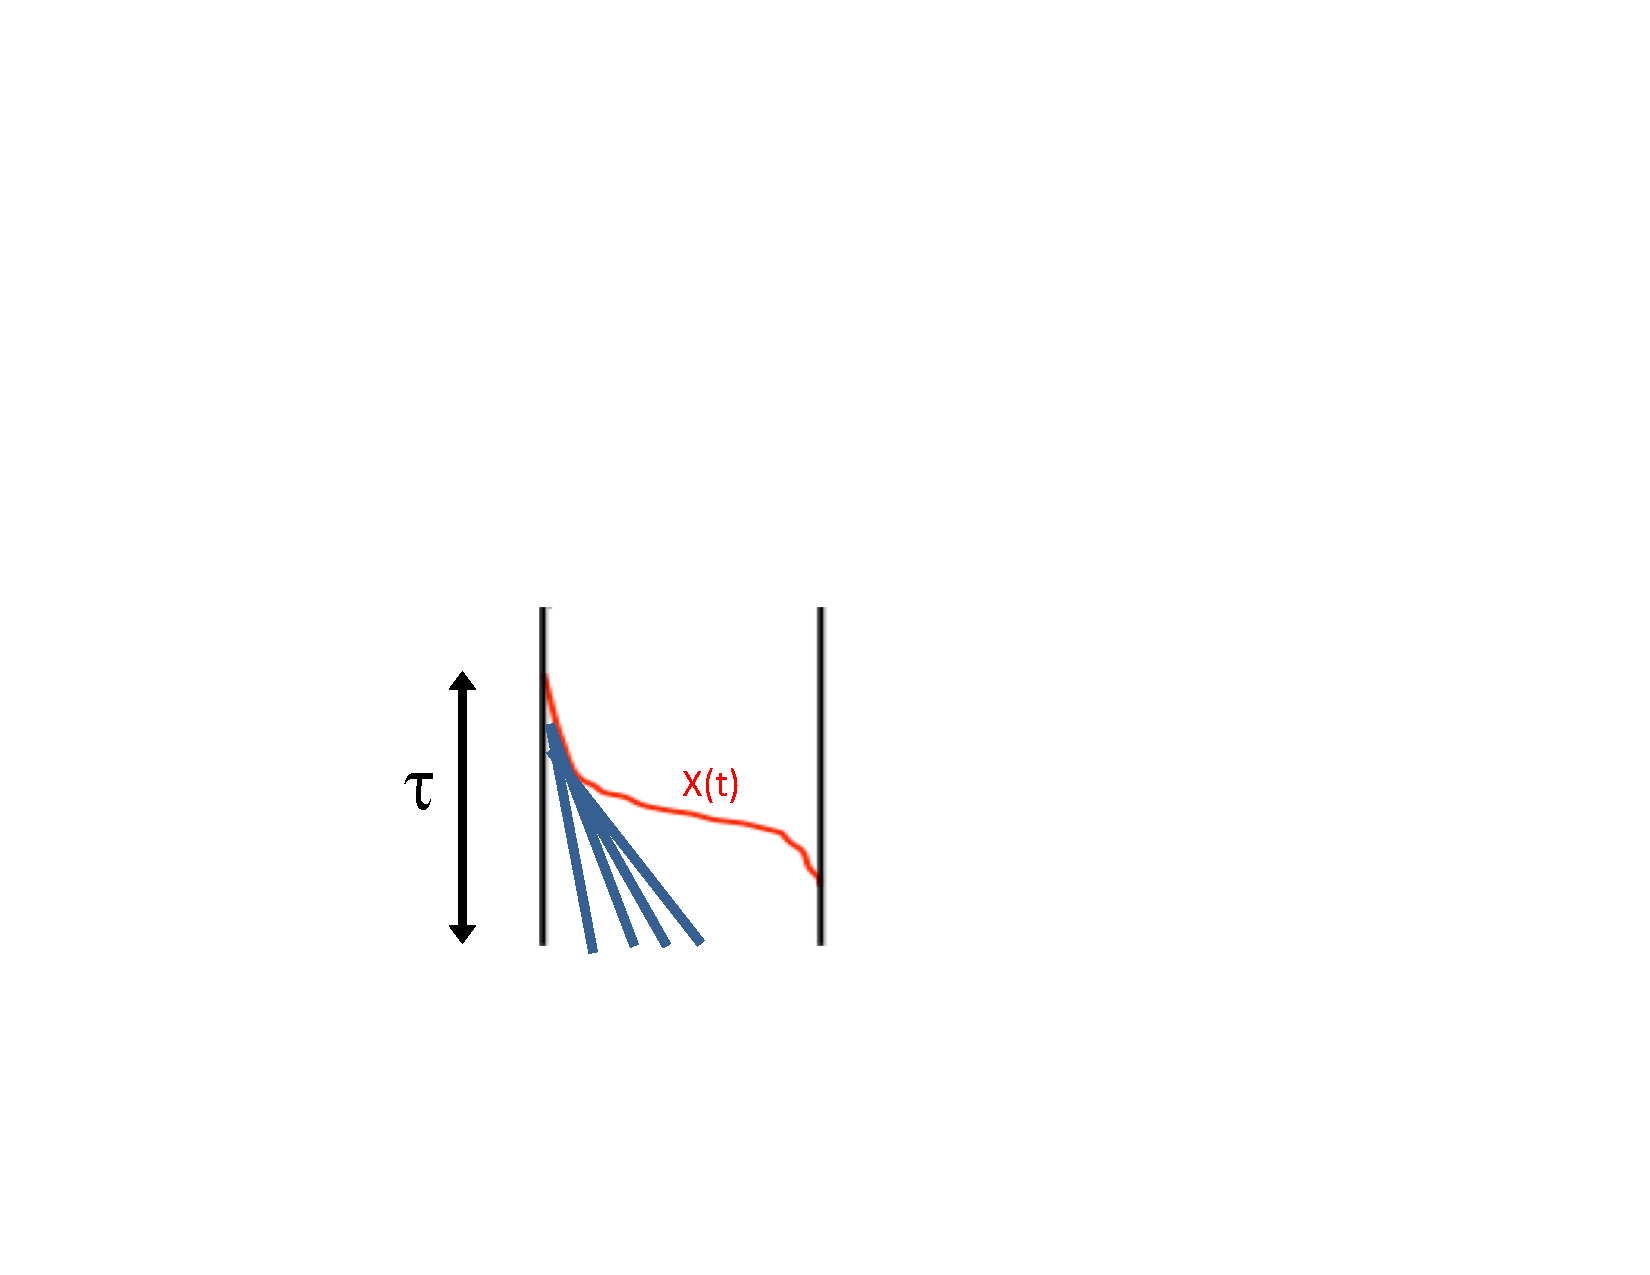
\includegraphics[width= 0.75 \textwidth]{figures/Hitchhiking/No_recom_coal.pdf}
\end{center}
\caption{The coalescent of 4 lineages, marked in blue, at a locus completed linked to our selected allele. The frequency trajectory of the selected allele $X(t)$ is shown in red.} \label{fig:no_recom_coal}
\end{marginfigure}
To better understand hitchhiking, first let's imagine examining variation at a locus fully linked
to our selected locus, just after our sweep reached fixation. Neutral alleles sampled at this locus
must trace their ancestral lineages back to the neutral
allele on whose background the selected allele initially arose (Figure
\ref{fig:no_recom_coal}). This is because
that background neutral allele, which existed $\tau$ generations ago, is the
ancestor of the entire population at this fully linked locus. Our individuals who
carry the beneficial allele are, from the perspective of these 
alleles, experiencing a rapidly expanding population. Therefore, a
pair of neutral alleles sampled at our linked neutral locus will be forced to
coalesce $\approx \tau$ generations ago. A newly derived allele with an additive selection coefficient $s$ will
take a time $\tau = 4\log(2N)/s$ generations to reach to fixation
within our population (see eqn. \eqref{eq:diploid_fix_time}). This is a very
short-time scale compared to the average neutral coalescent time of
$2N$ generations for a pair of alleles. Thus we expect little variation,
as few mutations will have arisen on these very short branches, and
those that have done will likely be singletons in our sample. \\

\begin{marginfigure}
\begin{center}
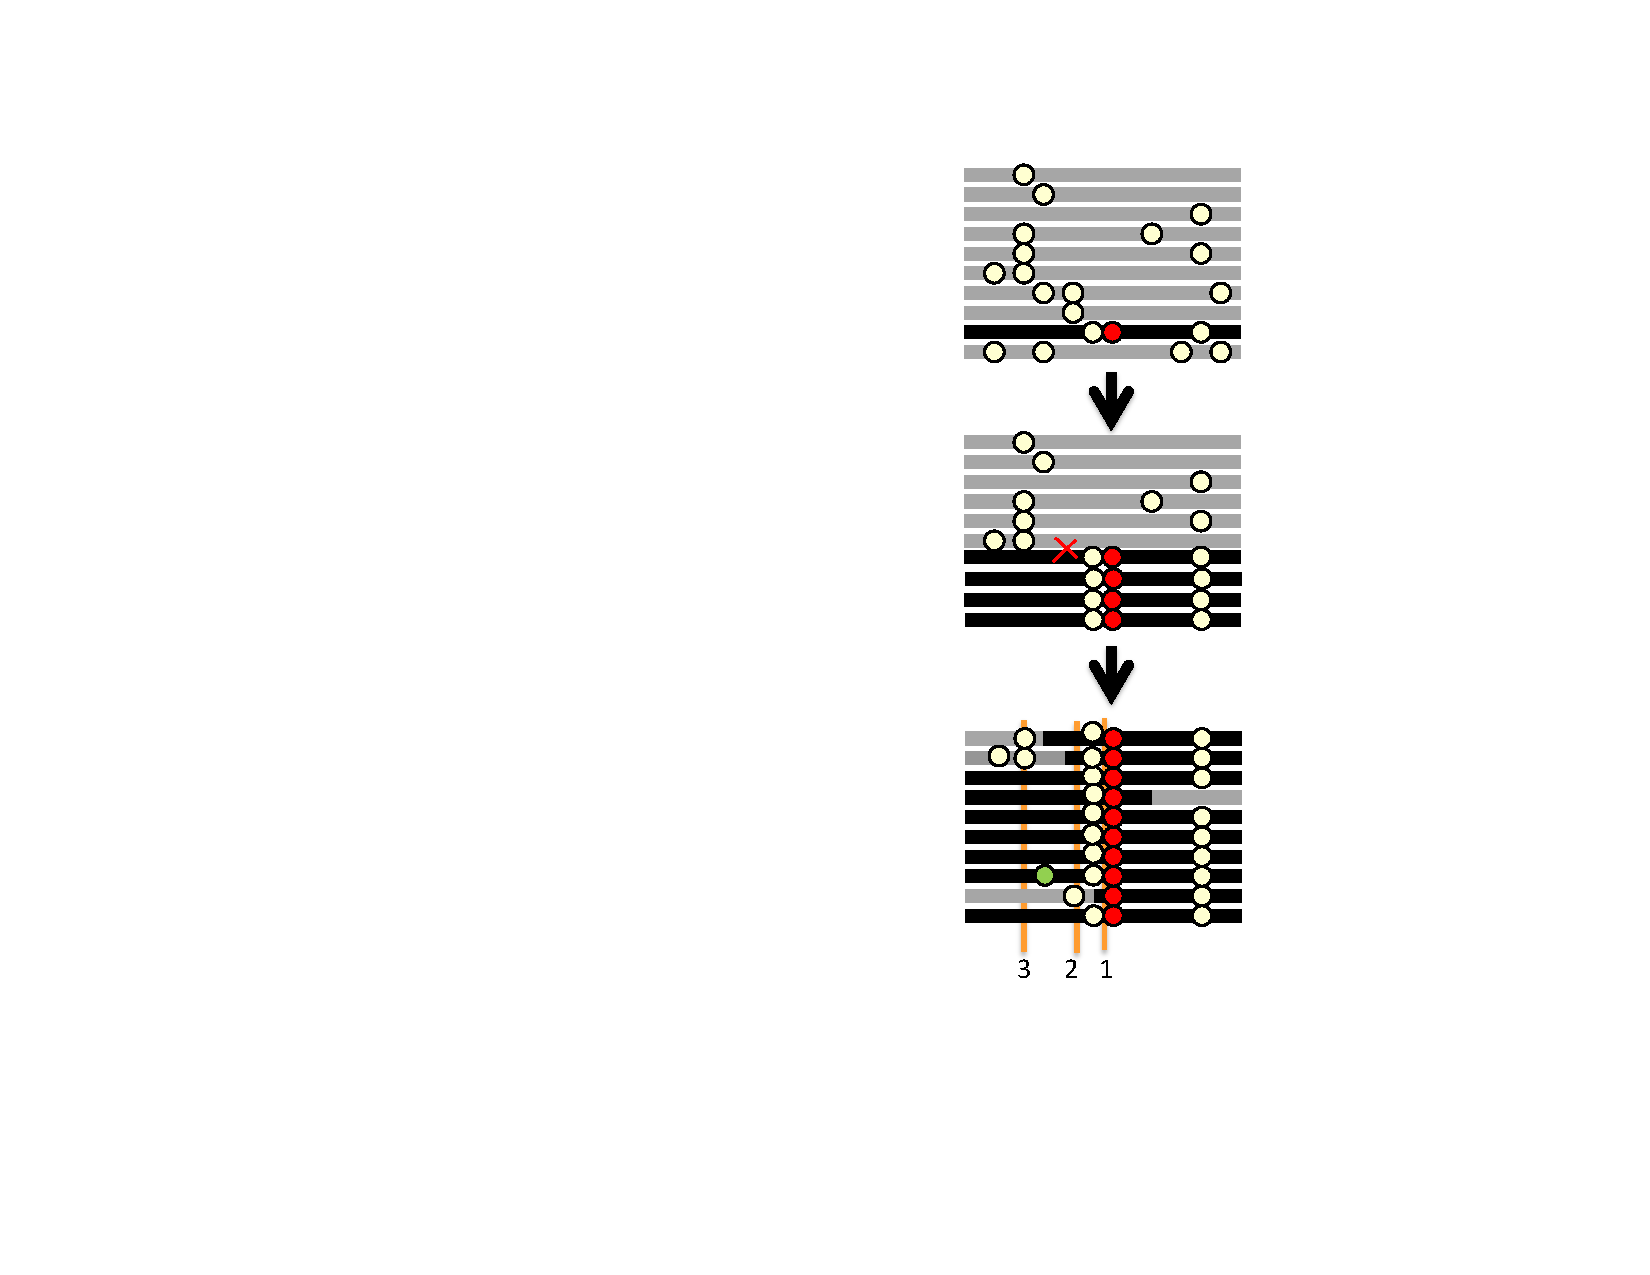
\includegraphics[width= 0.5 \textwidth]{figures/Hitchhiking/recom_haps_sweep.pdf}
\end{center}
\caption{A cartoon depiction of a sweep of a red beneficial allele over three time points. The haplotype that the beneficial arose on by mutation is shown in black. The three vertical orange lines mark the loci shown in Figure \ref{fig:sweep_haps_coal}. Neutral alleles segregating prior to the sweep appear as white circles, new mutations after the sweep as green circles.} \label{fig:sweep_haps}
\end{marginfigure}
Now let's think about a sweep in a recombining region. Again the
selected mutation arises on a particular haplotype, and it and its
haplotype starts to increase in frequency in the population. However,
now recombination events can occur between haplotypes carrying and not
carrying the selected allele, in individuals who are heterozygote for
the selected allele. These recombination events allow alleles that
were not present on the original selected haplotype to avoid being
swept out of the population, and also decouple the selected allele
somewhat from hitchhiking alleles, preventing many of them from hitchhiking all the way to fixation. Far out from the selected site, the recombination
rate is high enough that alleles that were present on the original
background barely get to hitchhike along at all, as recombination breaks up their association with the selected allele very rapidly.

\begin{figure}
\begin{center}
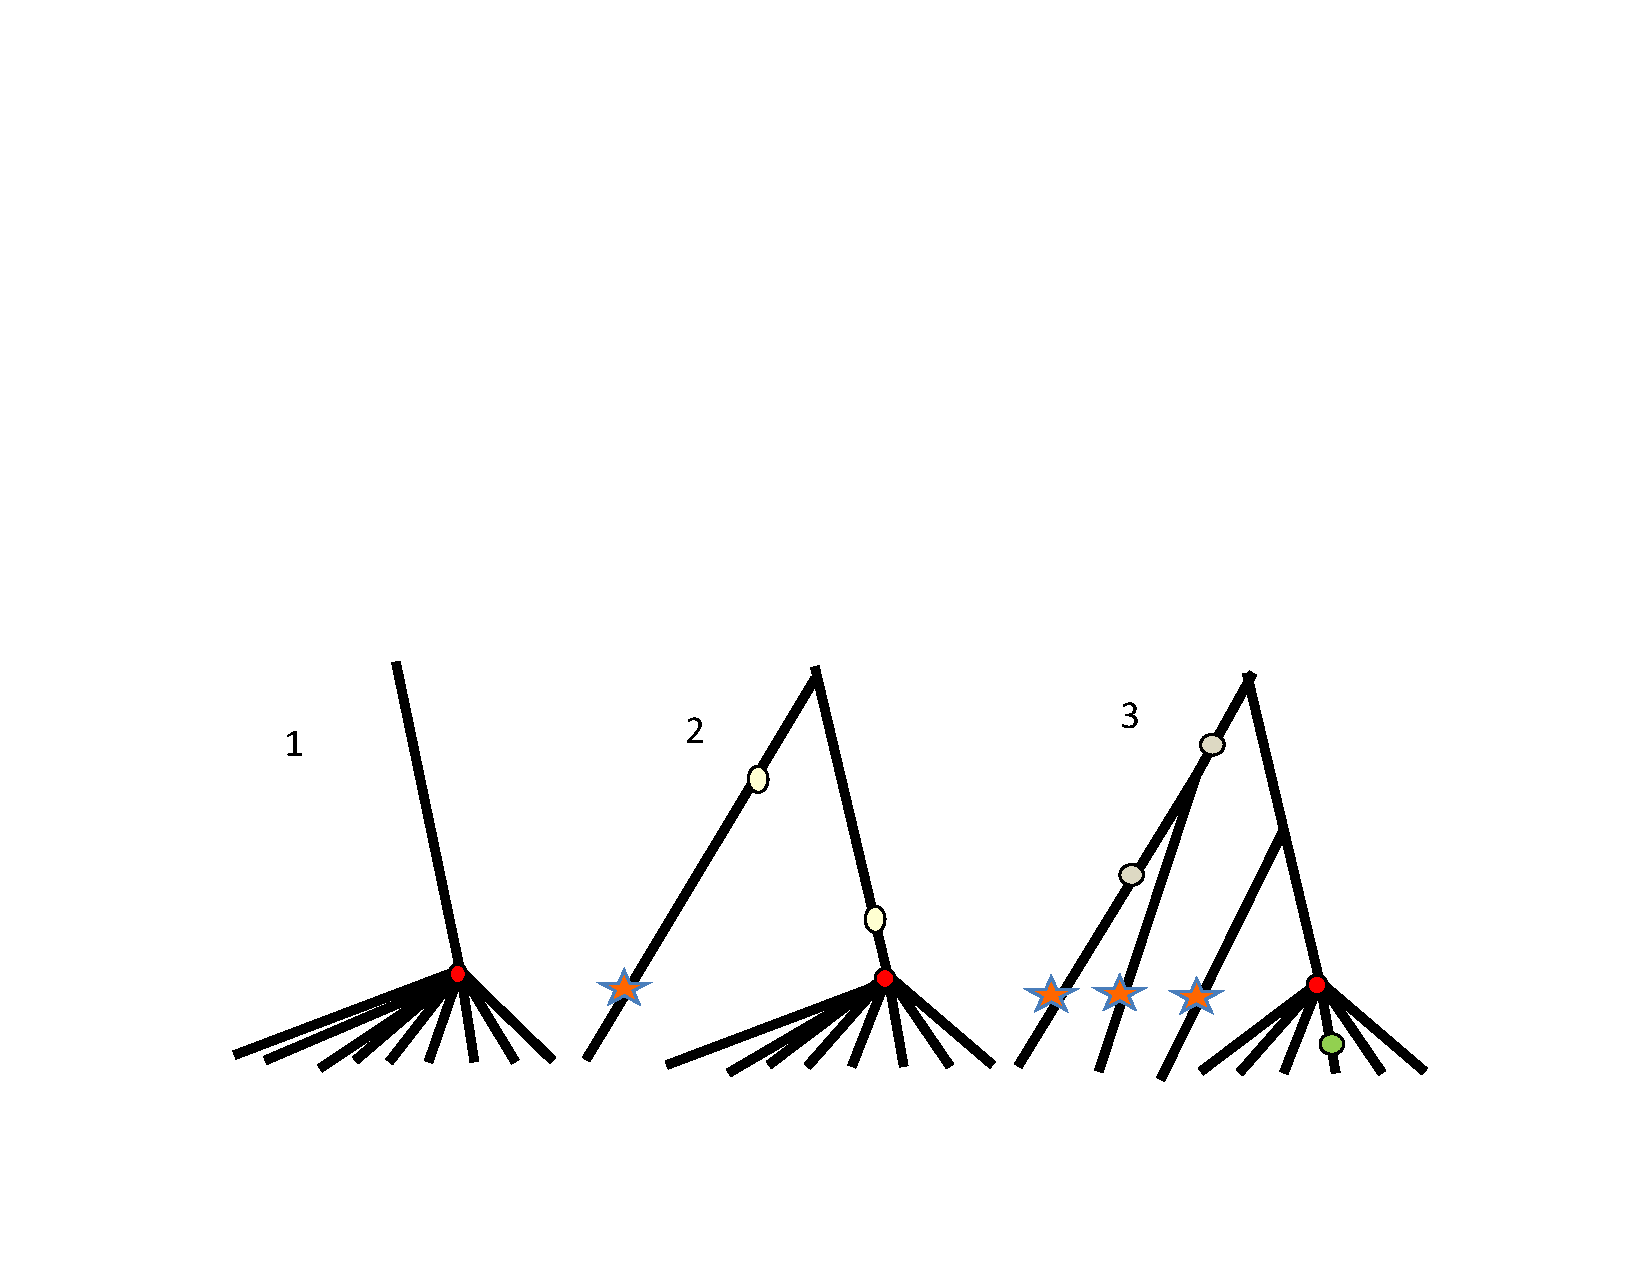
\includegraphics[width= 0.9 \textwidth]{figures/Hitchhiking/recom_haps_coal_sweep.pdf}
\end{center}
\caption{Coalescent genealogies at three loci different distances along the genome from a selective sweep. The locations of these three loci along the genome are marked in Figure \ref{fig:sweep_haps}. The selected mutation is shown in red. Lineages descended from recombination events during the sweep are marked in stars. Neutral mutations close to each of the loci are shown on the genealogy.} \label{fig:sweep_haps_coal}
\end{figure}

What do the coalesecent genealogies look like at loci various distances away from the
selected site? Well, close to the selected site all our alleles in the
present day trace back to a most recent common ancestral allele
present on that selected haplotype, and so are all forced to coalesce
around $\tau$ generations ago (locus 1). Slightly further out from the selected
site (locus 2), we have lineages that don't trace their ancestry back
to the original selected haplotype, but instead are descended from
recombinant haplotypes that recombined onto the sweep (the haplotype 2 from the
bottom). These lineages can coalesce neutrally with the other ancestral lineages
over far deeper time scales and mutations on these deeper lineages
correspond to the standing diversity present in our population
prior to the sweep. As we move even further out from the selected site
(locus 3), we encounter more and more lineages descended from
recombinant haplotypes that coalesce neutrally much deeper in time than $\tau$, 
allowing diversity to recover to background levels as we move away
from the selected site.

\begin{figure}
\begin{center}
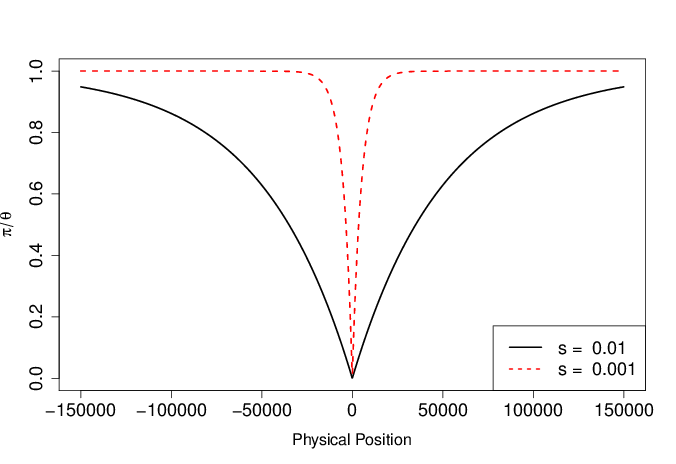
\includegraphics[width=0.75\textwidth]{figures/hitchhiking_reduction.png}
\end{center}
\caption{The expected reduction in diversity compared to its neutral expectation as
a function of the distance away from a site where a selected allele
has just gone to fixation. The sweeps associated with two different strengths of selection are shown, corresponding to a short timescale ($\tau$) for the sweep and long one. The recombination rate is $r_{BP}= 1\times
10^{-8}$.} \label{fig:hitchhiking_reduction}
\end{figure}



To model the expected pattern of diversity surrounding a selected site, we can think about a pair
of alleles sampled at a neutral locus a recombination distance $r$
away from our selected site. Our pair of alleles will be forced to
coalesce $\approx \tau$ generations if neither of them of are
descended from recombinant haplotypes.\\
\begin{marginfigure}
\begin{center}
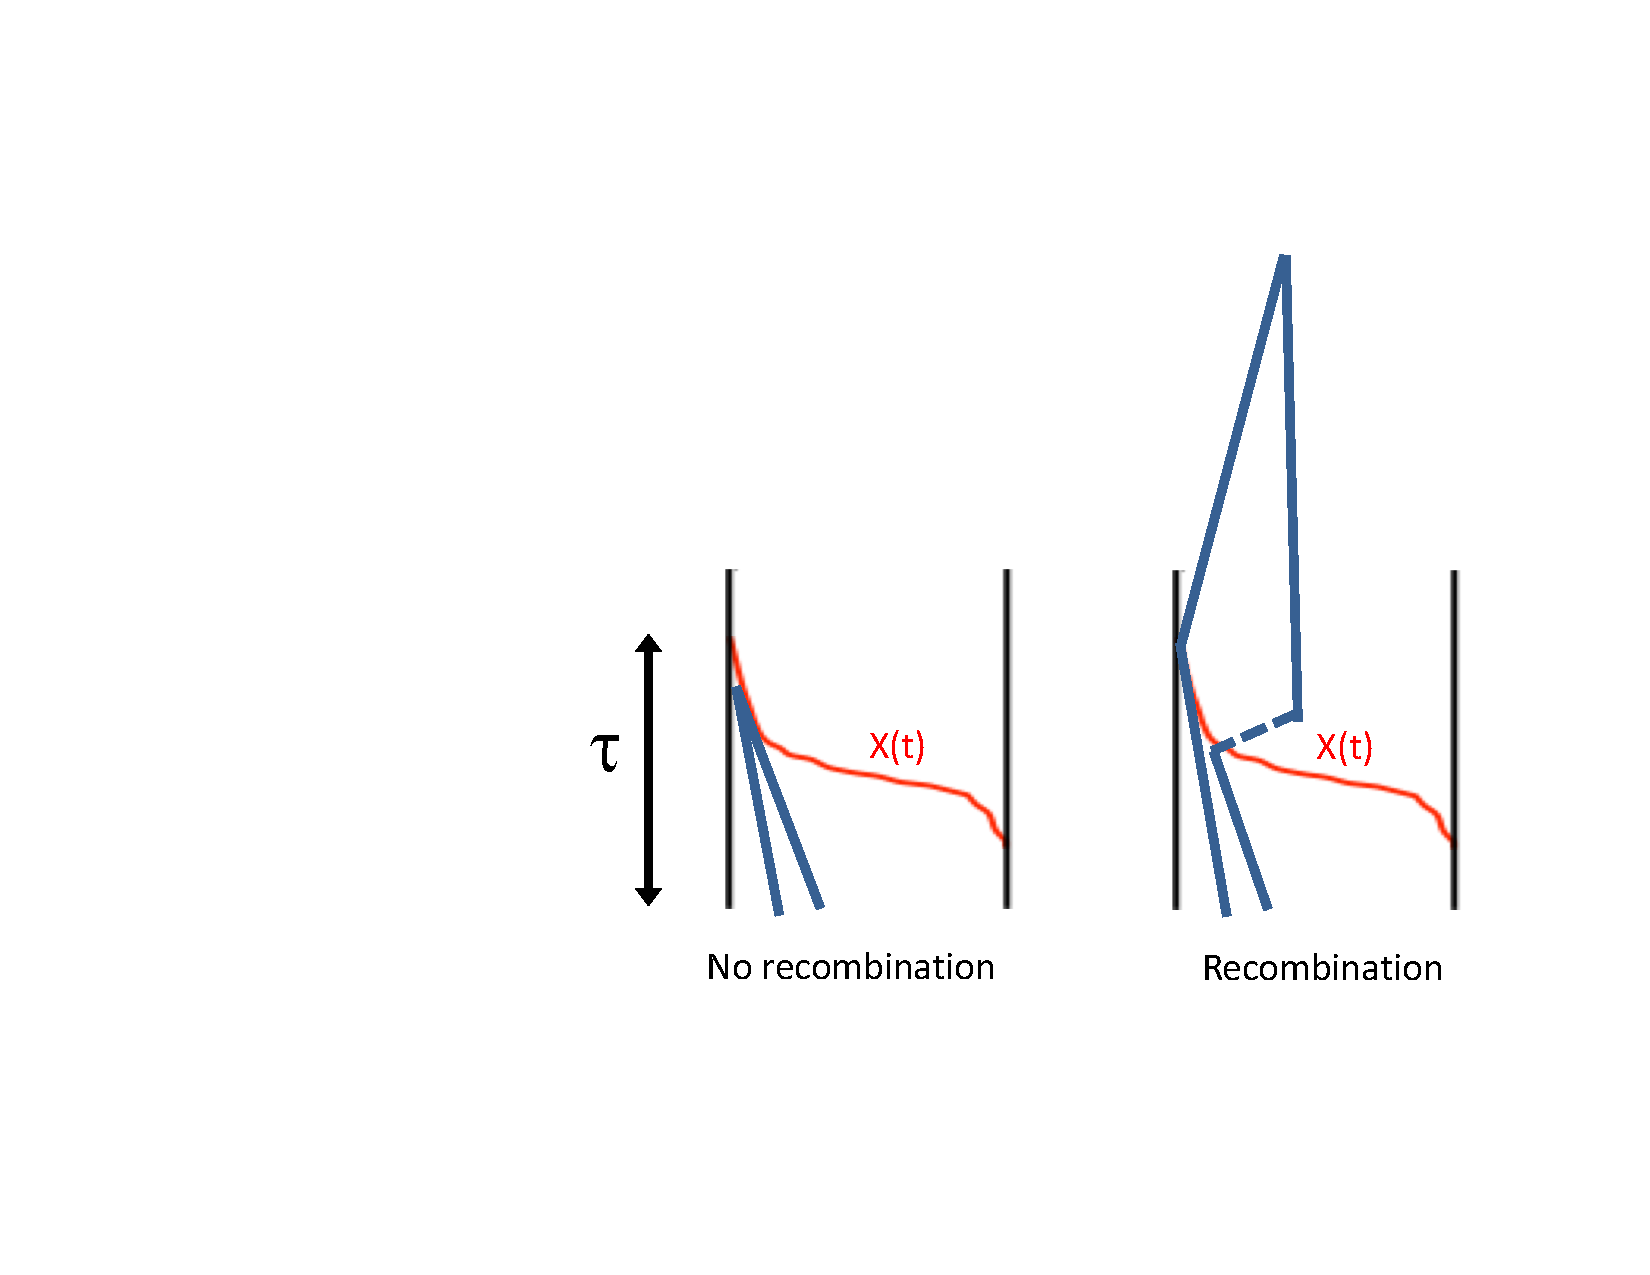
\includegraphics[width= \textwidth]{figures/Hitchhiking/Recom_coal.pdf}
\end{center}
\caption{} \label{fig:no_recom_coal}
\end{marginfigure}
We know that in the present day our neutral lineage is linked to
the selected allele. The probability that our lineage, in some
generation $t$ back in time, is in a heterozygote is $1-X(t)$, and the
probability that a recombination occurs in that individual is $r$. So
the probability that our neutral lineage is descended from a
recombinant haplotype $t$ generations back is 
\begin{equation}
r (1-X(t))
\end{equation}
So the probability ($p_{NR}$) that our lineage is not descended from a
recombinant haplotype 
from a recombination event in the
$\tau$ generations it takes our selected allele to move through the
population is
\begin{equation}
p_{NR}=\prod_{t=1}^{\tau} \big(1- r(1-X(j))\big)
\end{equation}
Assuming that $r$ is small, then $ \left(1- r(1-X(t))\right) \approx
e^{-r(1-X(t))}$,  such that
\begin{equation}
p_{NR}=\prod_{t=1}^{\tau} \left(1- r(1-X(t))\right) \approx \exp
\left( -r\sum_{t=1}^{\tau}
1- X(t) \right) =\exp
\left( -r \tau (1-\widehat{X}) \right)
\end{equation}
where
$\widehat{X}$ is the average frequency of the derived beneficial allele across its trajectory as it sweeps up in frequency,
$\widehat{X} = \frac{1}{\tau}  \sum_{t=1}^{\tau}
 X(t)$. As our allele is additive, its trajectory for frequencies
 $<0.5$ is the mirror image of its trajectory for frequencies $>0.5$, therefore its
average frequency $\widehat{X} =0.5$. This simplifies our expression to
\begin{equation}
p_{NR} = e^{-r \tau/2 }.
\end{equation}
The probability that neither of our lineages is descended from a
recombinant haplotype, and hence are forced to coalesce, is $p_{NR}^2$ (assuming that
they coalesce at a time close to $\tau$ so that they recombine
independently of each other for times $< \tau$).\\

If one or other of our lineages is descended from a recombinant haplotype, it will take them on average
$\approx 2N$ generations to find a common ancestor, as we are back to our
neutral coalescent probabilities. Thus, the expected time
till our pair of lineages find a common ancestor is
\begin{equation}
\E(T_2)  = \tau \times p_{NR}^2 +(1-p_{NR}^2) (\tau +2N) \approx
\left(1-p_{NR}^2 \right) 2N
\end{equation}
where this last approximation assumes that $\tau \ll 2N$. So the
expected pairwise diversity for neutral alleles at a recombination
distance $r$ away from the selected sweep ($\pi_r$) is
\begin{equation}
\E(\pi_r) = 2\mu \E(T_2)  \approx \pi_0 \left(1-e^{-r\tau} \right) \label{eqn:pi_HH}
\end{equation}
So diversity increases as we move away from the selected site,
slowly and exponentially plateauing to its neutral expectation $\pi_0$.\\
\begin{figure}
\begin{center}
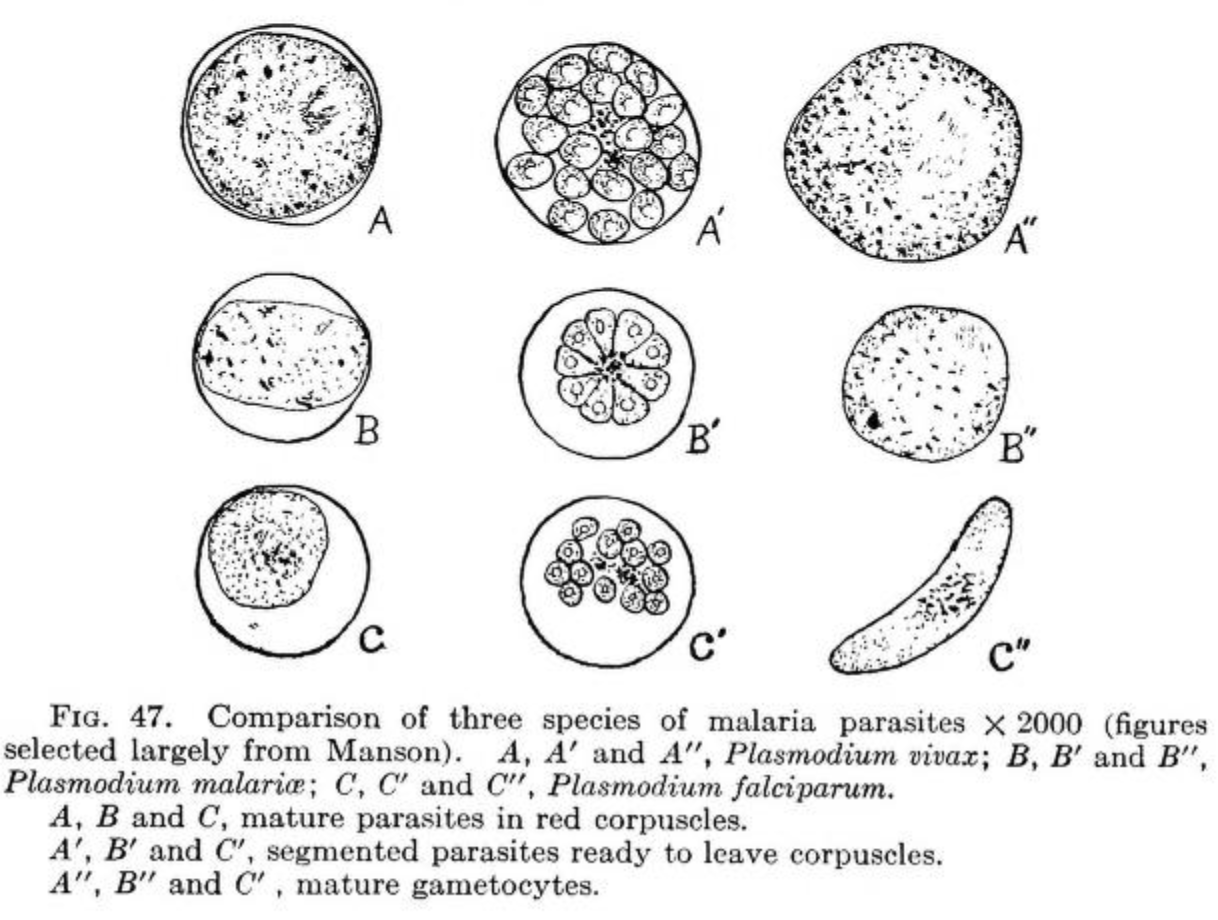
\includegraphics[width=\textwidth]{illustration_images/hitchhiking/malaria/malaria.png}
\end{center}
\caption{Three species of malaria parasites ({\it Plasmodium}) in red
  blood cells. Animal parasites and human disease (1918). Chandler, A.C. } \label{fig:malaria}
\end{figure}
The malaria pathogen ({\it Plasmodium falciparum}) has
evolved drug resistance to anti-malaria drugs, often by changes at
the dhfr gene. Figure \ref{fig:hitchhiking_malaria} shows levels of
genetic diversity (heterozygosity) at a set of markers moving out from the dhfr gene in a
set of  drug resistant malaria sequences collected in
Thailand \citep{nash2005selection}. We see the characteristic dip in diversity around the gene,
with zero diversity at a number of the loci very close to the gene,
suggesting a strong selective sweep. Fitting our simple model of a
sweep to this data,  we estimate that $\tau \approx 40$ generations,
corresponding to the drug-resistance allele fixing in very short time period. 
% these drug (Sulfadoxine–pyrimethamine) 

\begin{figure}
\begin{center}
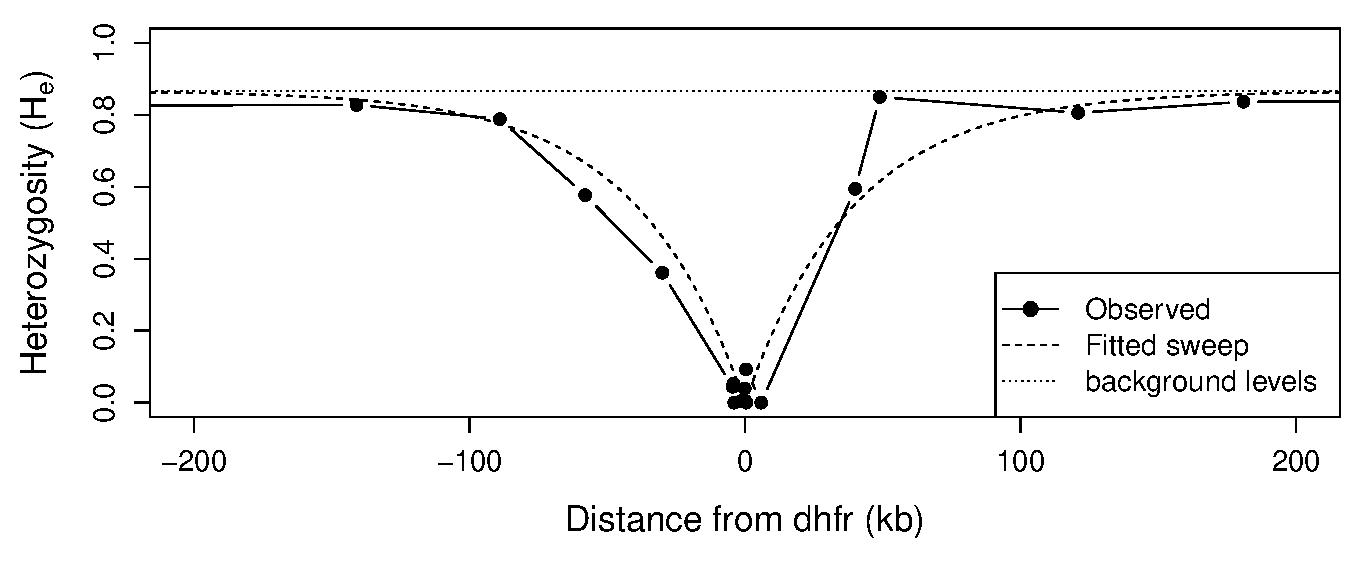
\includegraphics[width=\textwidth]{Journal_figs/recom_selection/malaria_sweep/dhfr_sweep.pdf}
\end{center}
\caption{Levels of heterozygosity at a set of microsatellite markers
  surounding the dhfr gene in samples of drug-resistant malaria ({\it Plasmodium falciparum}) from
  Thailand. The dotted horizontal line gives the average level of
  heterozygosity found at these markers in a set of drug-resistant
  malaria; we take this background as our $\pi_0$. Data from \citet{nash2005selection}. The dashed line shows
  our fitted hitchhiking model from equation \ref{eqn:pi_HH} with $\tau \approx 40$, fitted by
  non-linear least squares. The recombination rate in {\it P.
    falciparum} is $r_{BP}\approx 10^{-6}$bp$^{-1}$.} \label{fig:hitchhiking_malaria}
\end{figure}


To get a sense of the physical scale over which diversity is reduced,
consider a region where recombination occurs at a rate $r_{BP}$ per
base pair per generation, and a locus $ \ell $ base pairs away from the
selected site, such that $r=r_{BP } \ell $ (where $r_{BP}  \ell  \ll 1$ so we don't need to
worry about more than one recombination event occurring per
generation). Typical
recombination rates are on the order of $r_{BP} = 10^{-8}$. In Figure
\ref{fig:hitchhiking_reduction} we show the reduction in diversity,
given by eqn. \eqref{eqn:pi_HH}, for two different selection coefficients.\\ 

For our expected diversity level to recover to $50\%$ of
its neutral expectation $\E(\pi_r)/\theta=0.5$, requires a physical
distance $\ell^{*}$ such that $\log(0.5) = -r_{BP} \ell ^*\tau$, and by re-arrangement,
\begin{equation}
\ell^* = \frac{-\log(0.5)}{r_{BP} \tau }.
\end{equation}
As
$\tau$ depends inversely on the selection $s$ (eqn. \eqref{eq:diploid_fix_time}), the width of our trough of reduced diversity depends on $s/r_{BP}$.
All else being equal, we expect stronger sweeps or sweeps in regions of low
recombination to have a larger hitchhiking effect. For example, a selection coefficient of $s=0.1\%$ would reduce
diversity over 10's of kb, while a sweep of $s=1\%$ would affect
$\sim$100kb.   \\


\begin{question}
A recently published study has identified the genetic basis of
melanism in the pepper moth. This allele swept to fixation in northern
parts of the UK; a classic case of adaptation to industrial pollution
(made famous by the work of Kettlewell). The genetic basis of melanism
is a transposable element (TE) inserted into a pigmentation gene. The
investigators found that diversity is suppressed in a broad region
around the TE. Specifically, on the background of the TE, it takes
roughly 200 kb in either direction for diversity levels to recover to
50\% of genome-wide levels. \\

Random facts: In all moths and butterflies only males recombine;
chromosomes are transmitted without recombination in females. The
recombination rate in males is 2.9 cM/Mb.  Peppered moths have an
effective population size of roughly a hundred thousand
individuals. Kettlewell used to eat moths when out collecting them in
the field (personal communication, Art. Shapiro). \\
{\bf A)} Briefly explain how this pattern offers further evidence that the melanic allele was favoured by selection.\\
{\bf B)} Using this information, and assuming the allele's effects on fitness are additive, what is your estimate of the age of the allele? \\
{\bf C)} What is your estimate of the selection coefficient favouring this melanic allele?
\end{question}


\paragraph{Other signals of selective sweeps}
The primary signal of a recently completed selective sweep is the
characteristic reduction in diversity surrounding the selected site.
However, sweeps do leave other signals and these have also often been
used to identify loci undergoing selection. 
For example, neutral alleles further away from the selected site may
hitchhiking only part of the way to fixation if recombination occurs during
the sweep, which can lead to an excess of high-frequency
derived alleles at intermediate distances away from the selected site,
a pattern lasting for a short time after a sweep \citep{Fay:00,Przeworski:02,Kim:06}.
Also, as neutral diversity levels slowly recover through an influx of
new mutations after a sweep, there is a strong skew towards low
frequency derived alleles, a pattern that persists for many
generations \citep{Braverman:95, Przeworski:02,Kim:06}. The excess of
rare alleles, compared to a neutral model, can be captured by statistics such as Tajima's D (which
we encountered back in our discussion of the neutral site frequency eqn
\ref{eqn_Tajimas_D}). Thus one way to look for loci that have undergone selective sweeps is to calculate Tajima's D from data in
windows along the genome and look for
strong departures from the null distribution.


\begin{figure}
\begin{center}
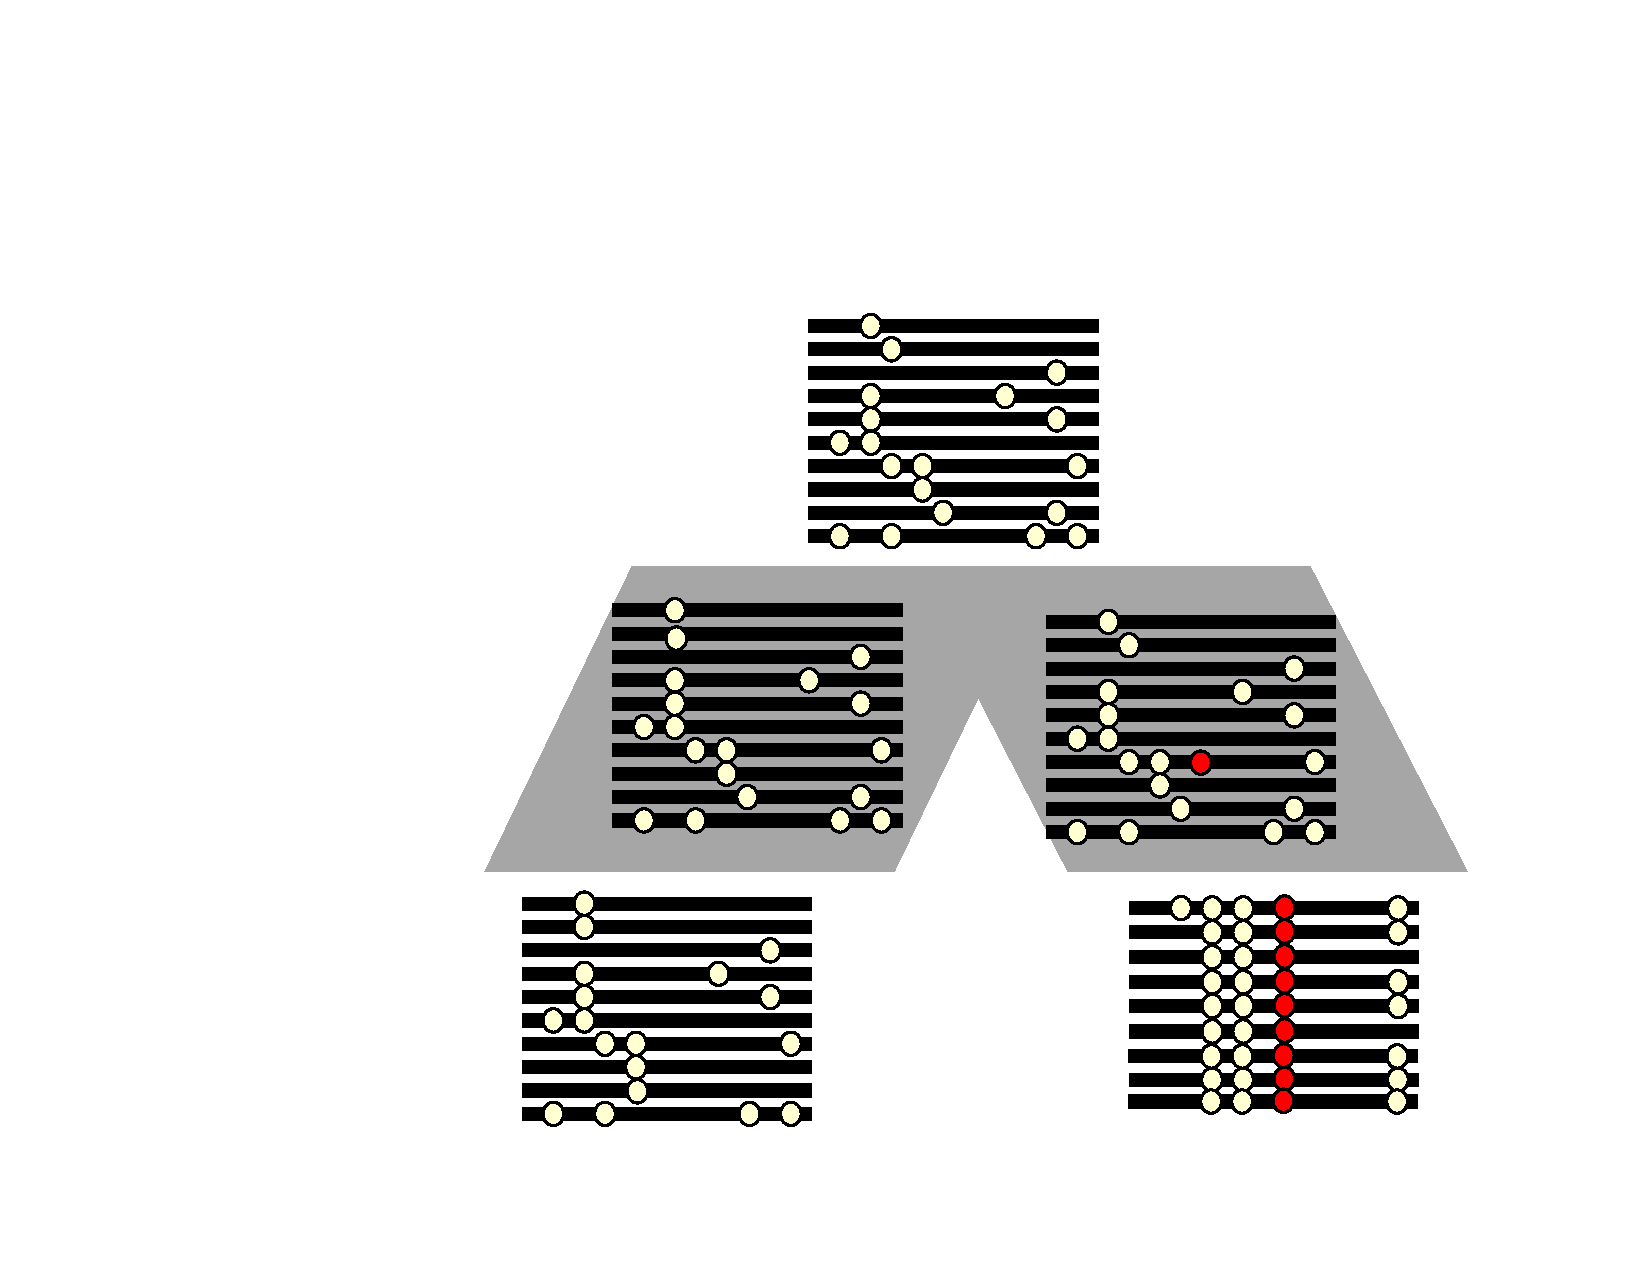
\includegraphics[width=0.5 \textwidth]{figures/Hitchhiking/two_pops_sweep.pdf}
\end{center}
\caption{Two populations descended from a common ancestral
  population. A beneficial mutation has occurred in population and
  swept to fixation.} \label{fig:local_sweep_haps}
\end{figure}

We can also use comparisons among multiple populations to look for evidence of sweeps occurring in one of the
populations, for example to identify alleles involved in local adaptation (see \ref{fig:local_sweep_haps}). A selective sweep will decrease the within-population diversity ($H_S$)
surrounding the selected site, without affecting the diversity between different
populations. Thus local sweeps create peaks of
$\fst$ between weakly differentiated populations. 

\citet{hohenlohe2010population} studied genome-wide patterns of
$\fst$ between marine and freshwater populations of  threespine
stickleback ({\it Gasterosteus aculeatus}). 
Between different marine populations, they found no strong peaks of $\fst$;
however, between the marine and freshwater comparisons they found a
number of high $\fst$  peaks that were replicated over a number of
freshwater-marine comparisons. They identified a number of novel
regions responsible for the adaptation of sticklebacks to freshwater
environments and also a number of loci previously identified in crosses between marine and freshwater populations. For example, the first peak of Linkage
Group IV includes Ectodysplasin A (Eda), a gene involved in the adaptive loss of armour plating in freshwater environments.
\begin{figure}
\begin{center}
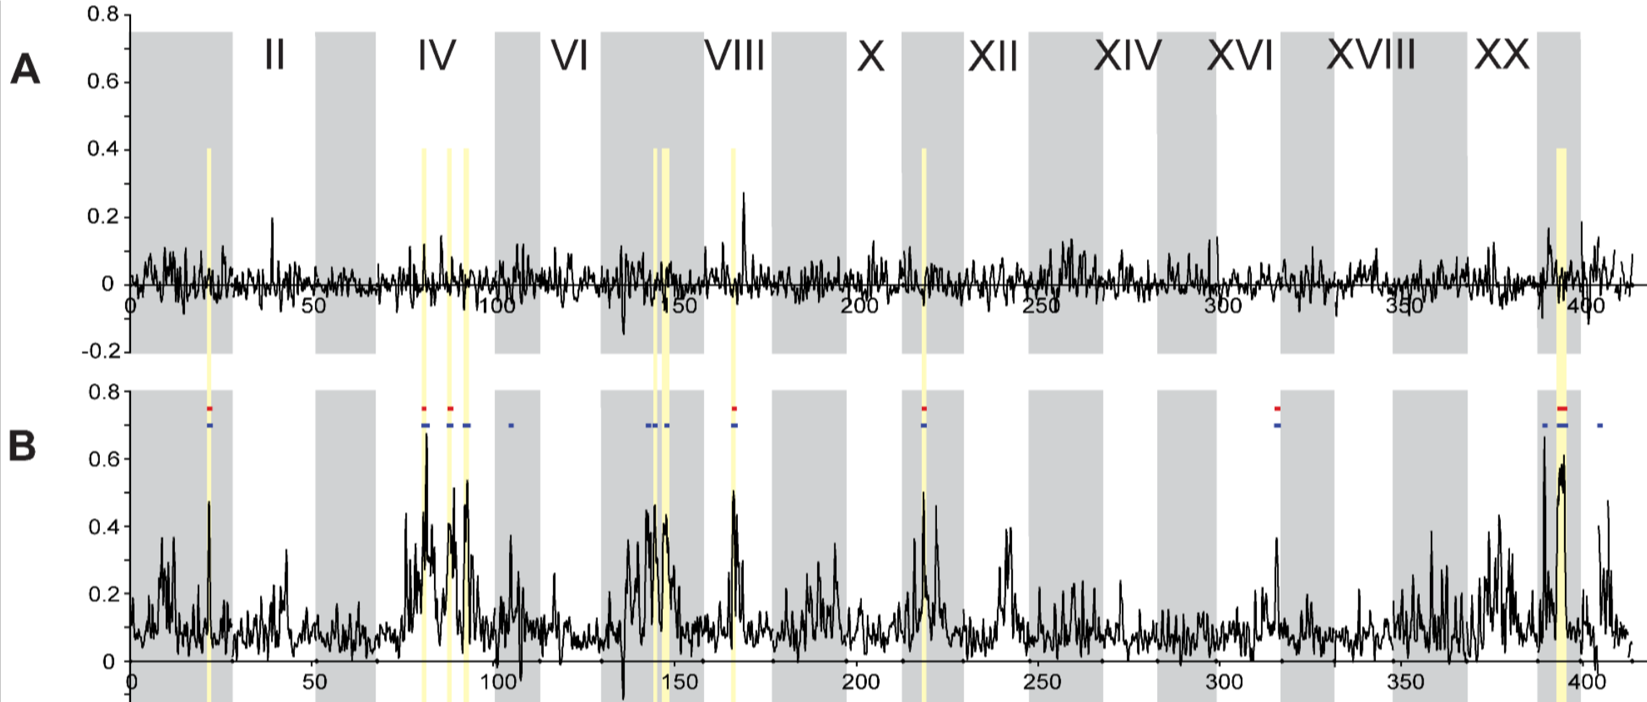
\includegraphics[width=0.9 \textwidth]{Journal_figs/recom_selection/Stickleback_FST/hohenlohe.png}
\end{center}
\caption{$\fst$ across the stickleback genome, with colored bars indicating
  significantly elevated ($p \leq 10^{−5}$, blue; $p \leq 10^{−7}$,
  red) and reduced ($p \leq 10^{−5}$, green) values. The alternating
  white and grey panels indicate different linkage groups. {\bf A)} $\fst$
  between two oceanic populations {\bf B)} Average $\fst$ between a
  freshwater population and the two marine populations. Figure and
  caption text from \citet{hohenlohe2010population}.} \label{fig:local_sweep_haps}
\end{figure}


\paragraph{Soft Sweeps from multiple mutations and standing variation.}
In our sweep model above, we assumed that selection favoured a
beneficial allele from the moment it entered the population as a
single copy mutation  (left panel, Figure \ref{fig:soft_sweep_haps}). However, when a novel selection pressure
switches on, multiple mutations at the same gene
may start to sweep, such that no one of these alleles sweeps
to fixation (middle panel, Figure \ref{fig:soft_sweep_haps}). These sweeps involving multiple mutations significantly
soften the impact of selection on genomic diversity, and so are called 'soft sweeps'.

\begin{figure}
\begin{center}
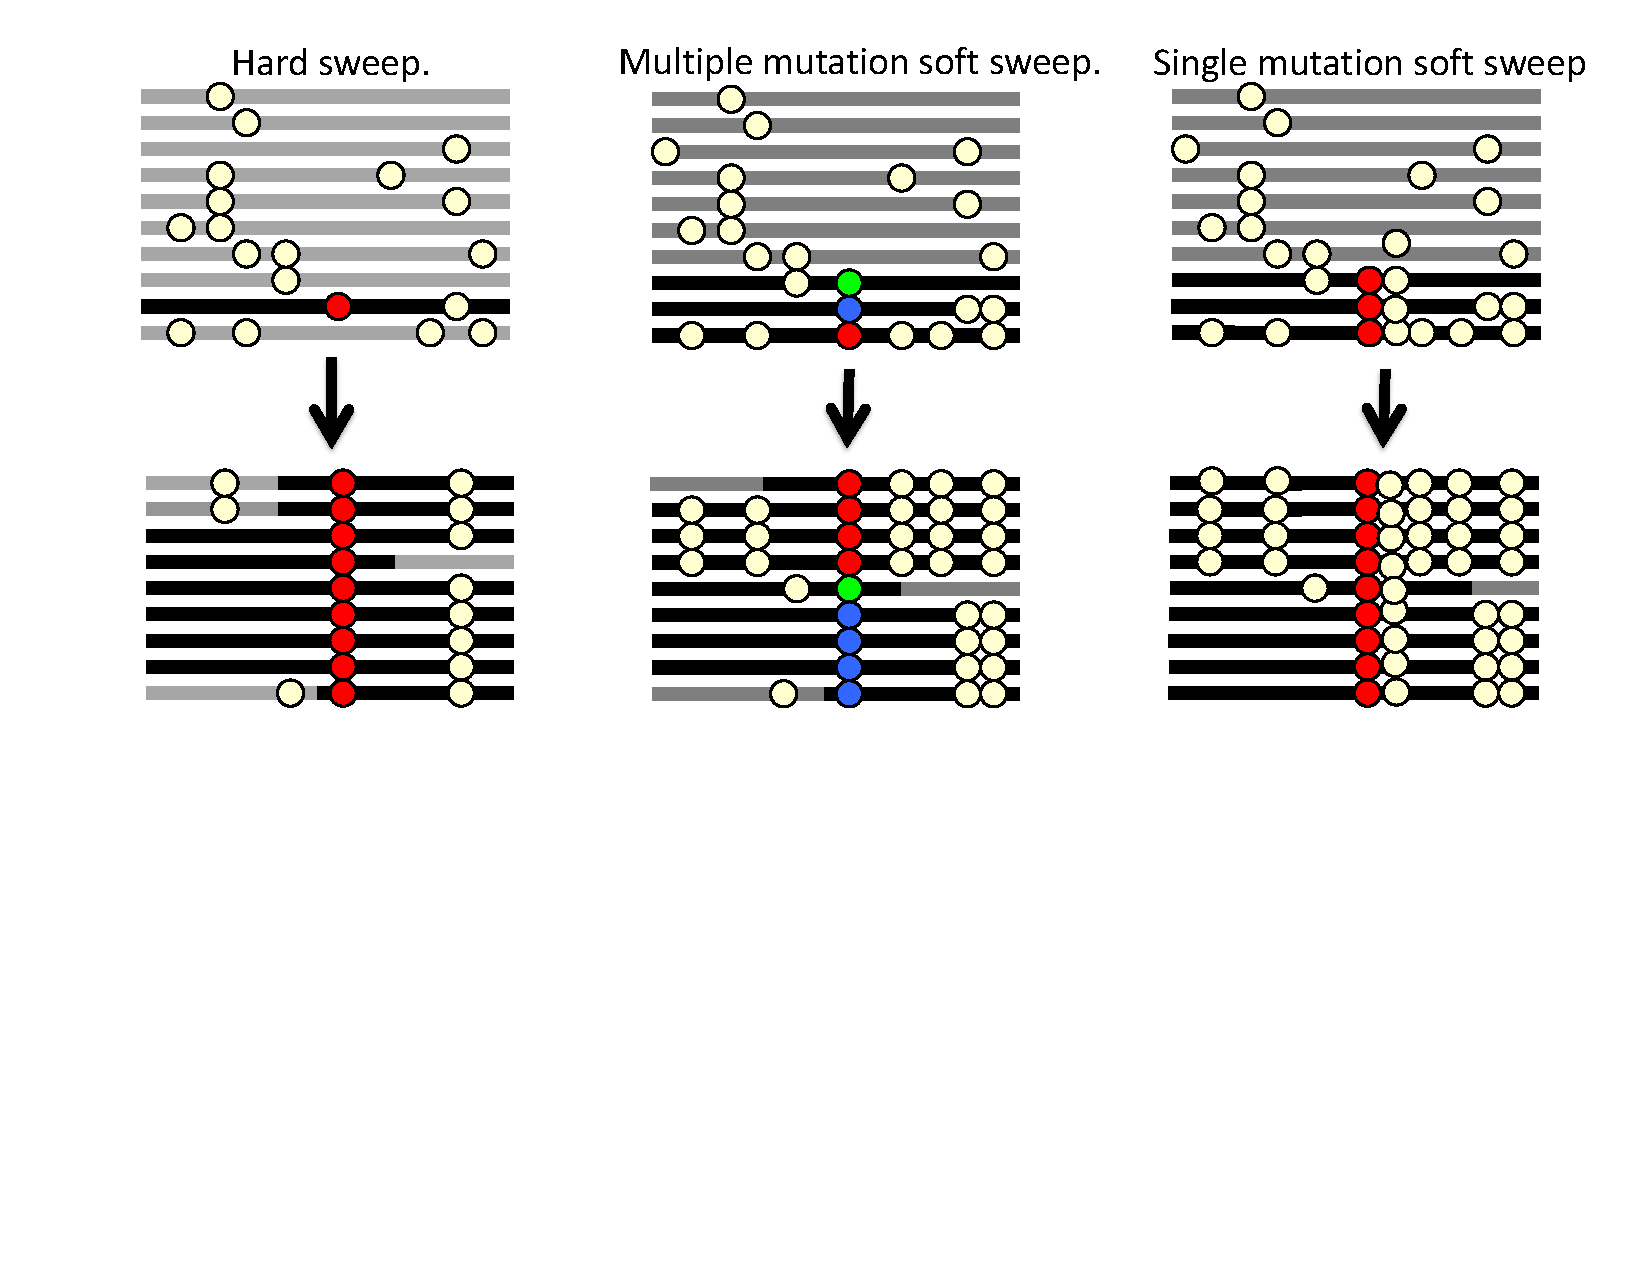
\includegraphics[width=\textwidth]{figures/Hitchhiking/Soft_sweeps.pdf}
\end{center}
\caption{Three types of sweeps. } \label{fig:soft_sweep_haps}
\end{figure}

Another way that the impact of a sweep can be softened is if our
allele was segregating in the population for some time before it
became beneficial. That additional time means that our allele can have
recombined onto various haplotype backgrounds, such that when
selection pressures switch, the selected allele sweeps up in frequency on 
multiple different haplotypes (right panel, Figure \ref{fig:soft_sweep_haps}). 
Detecting and differentiating these different types of sweeps is an active area of
empirical research and theory in population genomics (see \citet{hermisson2017soft} for an overview of
developments in this area).

%For example recall the multiple mutations at G6PD
%in the prior chapter. 

\section{The genome-wide effects of linked selection.}

To what extent are patterns of variation along the genome and
  among species shaped by linked selection, such as selective sweeps? 
We can hope to identify individual cases of strong selective sweeps
along the genome, but how do they contribute to broader patterns of
variation?

 Two observations have puzzled population geneticists since the
inception of molecular population genetics. The first is the relatively high
level of genetic variation observed in most obligately sexual species.  
The neutral theory of molecular evolution was developed in part to
explain these high levels of diversity. As we saw in Chapter \ref{Chapter:Drift}, 
under a simple neutral model, with constant population size, we should expect the amount of neutral genetic
diversity to scale with the product of the population size and
mutation rate. The second observation, however, is the relatively narrow range 
of polymorphism across species with vastly different census sizes (see
Figure \ref{fig:Leffer} and \citet{leffler:12} for a recent review). 
As highlighted by \citet{Lewontin:74} in his discussion of the paradox
of variation, this observation seemingly contradicts the prediction of the neutral theory that
genetic diversity should scale with the census population size. There are a number of explanations for the discrepancy between genetic
diversity levels and census population sizes. The first is that the effective size of the population ($N_e$) is
often much lower than the census size, due to high variance in
reproductive success and frequent bottlenecks (as discussed in  Chapter \ref{Chapter:Drift}). 
The second major explanation, \erin{this citation is coming through as a question mark in the text..} put forward by \citet{MaynardSmith:74},
is that neutral levels of diversity are also systematically reduced by the effects of linked selection. 
In large populations, selective sweeps and other forms of linked selection may come to dominate over genetic drift as a
source of stochasticity in allele frequencies, potentially establishing an upper limit to levels of diversity \citep{Kaplan:89, Gillespie:00}. 

\begin{figure}
\begin{center}
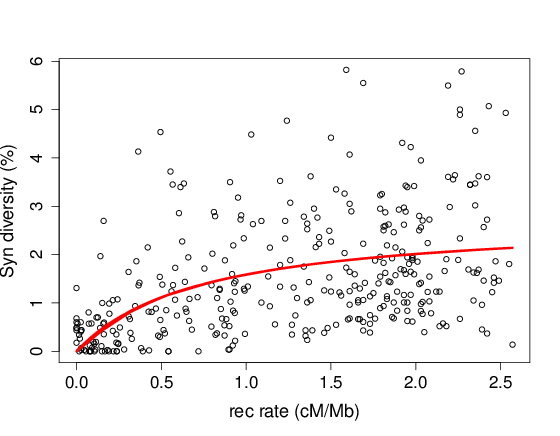
\includegraphics[width=0.75\textwidth]{figures/Genomewide_HH.png}
\end{center}
\caption{The relationship between (sex-averaged) recombination rate and synonymous
  site pairwise diversity ($\pi$) in {\it Drosophila melanogaster}
  using the data of \citep{Shapiro:07} (kindly provided by Peter
  Andolfatto, see \citet{sella2009pervasive} for details). The curve is the
  predicted relationship between $\pi$ and recombination rate, obtained
  by fitting equation \eqref{eqn:pi_GW_HH} to this data 
 using non-linear least squares via the {\tt nls()} function in {\tt R}.} \label{fig:GW_hitchhiking_reduction}
\end{figure}

One strong line of evidence for the action of linked selection in reducing levels of
polymorphism is the positive correlation between putatively
neutral diversity and recombination seen in a number of species, as, all
else being equal, linked selection should remove diversity more quickly in regions of low recombination 
\citep{Aguade:89,Begun:92,Wiehe:93,Cutter:10,Hellmann:08,Cai:09,
  cutter2013}. For example, {\it Drosophila melanogaster} diversity
levels are much lower in genomic regions of low recombination (see
Figure \ref{fig:GW_hitchhiking_reduction}). This pattern can not be
explained by differences in mutation rate between low and high
recombination regions as this pattern is not seen strongly in
divergence data among species.

These patterns could reflect the action of selective sweeps happening
recurrently along the genome. In the next section we'll present a model for how levels of
genetic diversity should depend on recombination and the density of
functional sites under a model of recurrent selective sweeps.
However, other forms of linked selection can impact genetic
diversity in similar ways. For example, linked genetic diversity is
continuously lost from natural populations due to the removal of
haplotypes that carry deleterious alleles
\citep{Charlesworth:95,Hudson:95}; this is called the 'background selection'
model. Below we'll discuss the background selection model and its
basic predictions.

%,Neher:13,Good:14
More generally, a wide range of models of selection predict the removal of neutral
diversity linked to selected sites. This is because the diversity-reducing effects of high variance in reproductive success are compounded over the generations when there is heritable variance in fitness 
\citep{Robertson:61,Santiago:95,Santiago:98,Barton:00}.  Many
different modes of linked selection likely contribute to these
genome-wide patterns of diversity; the present challenge is how to
differentiate among these different modes.


\subsection{A simple recurrent model of selective sweeps}
To explain how a constant influx of sweeps could impact levels of
diversity, here we will develop a model of recurrent
selective sweeps.

Imagine we sample a a pair of neutral alleles at a locus a genetic distance $r$ away from a locus where
sweeps are initiated within the population at some very low rate $\nu$
per generation. The waiting time between sweeps
at our locus is exponentially distributed $\sim Exp(\nu)$. Each sweep rapidly transits through the population in $\tau$
generations, such that each sweep is finished long before the next
sweep ($\tau \ll \nicefrac{1}{\nu}$). \\

As before, the chance that our neutral lineage fails to recombine
off the sweep is $p_{NR}$, such that the probability that
our pair of lineages are forced to coalesce by a sweep is $e^{-r \tau}$. Our
lineages therefore have a very low probability
\begin{equation}
\nu e^{-r \tau}
\end{equation}
of being forced to coalesce by a sweep per generation. If our lineages do not coalesce due to a sweep, they coalesce at a neutral rate of $\nicefrac{1}{2N}$ per generation. Thus the average
waiting time till a coalescent event between our neutral pair of
lineages due to either a sweep or a neutral coalescent event is
\begin{equation}
\E(T_2) = \frac{1}{\nu e^{-r \tau} + \nicefrac{1}{2N}}
\end{equation}

Now imagine that the sweeps don't occur at a fixed location with
respect to our locus of interest, but now occur uniformly at random
across our \ec{genome}. The sweeps are initiated at a very low rate of
$\nu_{BP}$ per basepair per generation. The rate of coalescent due to
sweeps at a locus $\ell$ basepairs away from our neutral loci is
$\nu_{BP} e^{-r_{BP} \ell \tau}$. If our neutral locus is in the
middle of a chromosome that stretches $L$ basepairs in either direction,
the total rate of sweeps per generation that force our pair of lineages to coalesce is
\begin{equation}
2\int_0^{L} \nu_{BP} e^{-r_{BP} \ell \tau} d \ell =
\frac{2\nu_{BP}}{r_{BP} \tau} \left(1-e^{-r_{BP} \tau L} \right)
\end{equation}
so that if $L$ is very large ($r_{BP} \tau L \gg 1$), the rate of coalescence per
generation due to sweeps is $\nicefrac{2\nu_{BP}}{r_{BP} \tau}$. The total rate
of coalescence for a pair of lineages per generation is then
\begin{equation}
\frac{2\nu_{BP}}{r_{BP} \tau}+\frac{1}{2N}
\end{equation}
So our average time till a pair of lineages coalesce is
\begin{equation}
\E(T_2) = \frac{1}{\nicefrac{2\nu_{BP}}{r_{BP} \tau}+\nicefrac{1}{2N}} = \frac{r_{BP}2N}{\nicefrac{4N\nu_{BP}}{ \tau}+r_{BP}}
\end{equation}
such that our expected pairwise diversity ($\pi=2\mu\E(T_2)$) in a region of
recombination rate $r_{BP}$ that experiences sweeps at rate $\nu_{BP}$
is  
\begin{equation}
\E(\pi) = \theta \frac{r_{BP}}{\nicefrac{4N\nu_{BP}}{ \tau}+r_{BP}} \label{eqn:pi_GW_HH}
\end{equation}
The expected diversity increases with $r_{BP}$, as higher recombination rates decrease the likelihood of being forced to coalesce by a sweep. Expected diversity decreases with $\nu_{BP}$, as a greater density of functional sites increases the chance of experiencing a nearby sweep. As we move to high $r_{Bp}$, assuming that $\nu_{BP}$ doesn't increase with $r_{BP}$, our level of diversity should plateau to $\theta$, the level of genetic diversity of a neutral site completely unlinked to any selected loci. An example of fitting this curve to data is shown in Figure \ref{fig:GW_hitchhiking_reduction}. 
%Assuming that the density of functional sites experiencing sweeps ($\nu+{BP}$) remains the same across recombination environments, i.e. that $r_{BP}$ and $\nu_{BP}$ are uncorrelated 

\subsection{Background selection}

% \citep{sella2009pervasive}
Populations experience a constant influx of
deleterious alleles at functional loci, while selection acts to purge
them from the population, maintaining levels of constraint at these loci. As
we discussed in Chapter \ref{Chapter:OneLocusSelection}, this results
in a constant level of deleterious variation in the population. The
constant selection against this deleterious variation has effects on diversity at linked
sites. Each deleterious mutation arises at random on a haplotype in the
population, \ec{and as selection purges this mutation, it removes with it any neutral alleles that were on this
haplotype}. This constant removal of linked alleles from the population
acts to reduce diversity in regions surrounding functional loci \citep{Hudson:95b,Nordborg:96}. 

\begin{figure}
\begin{center}
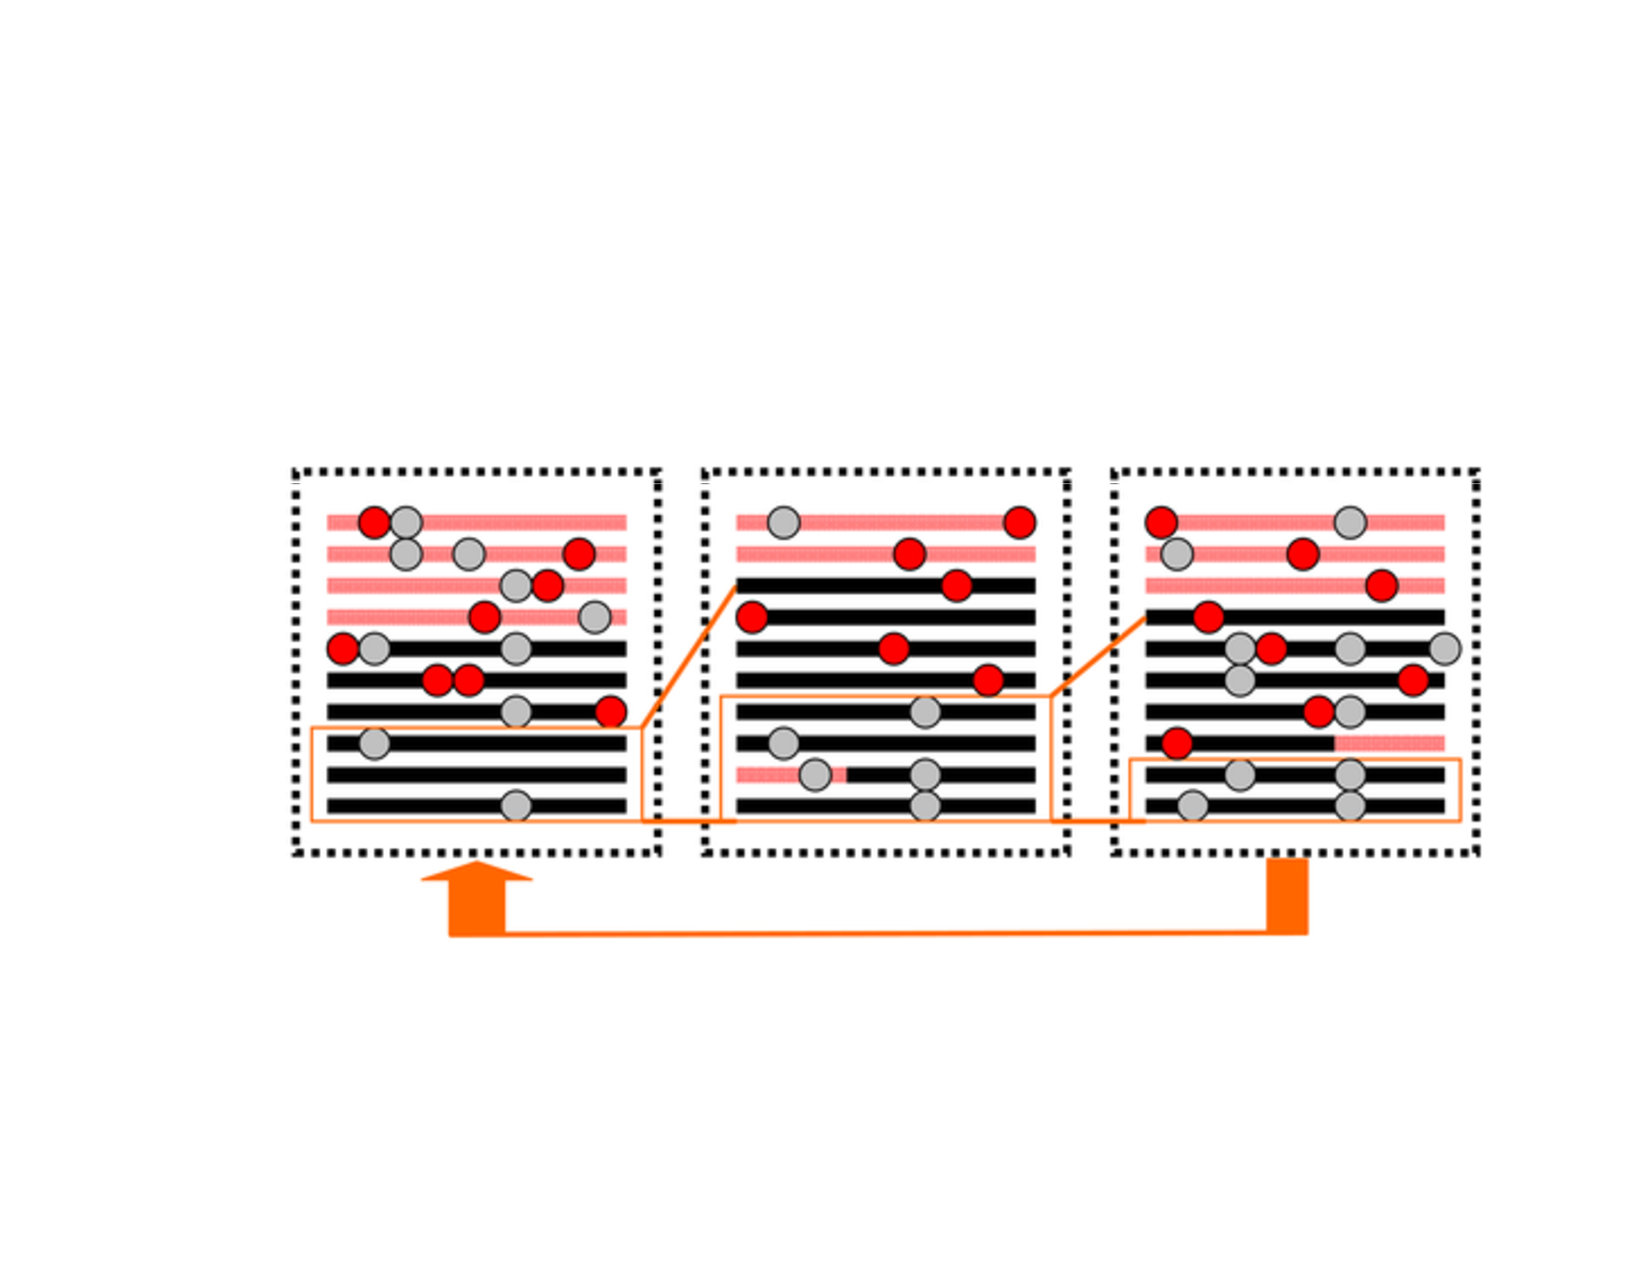
\includegraphics[width=0.75 \textwidth]{figures/Hitchhiking/BGS_cartoon.pdf}
\end{center}
\caption{A cartoon depiction of a region for 10 haplotypes
  experiencing background selection. Neutral mutations are shown as
  gray circles, and deleterious mutations in red. Over time,
  chromosomes carrying deleterious mutations are removed from the
  population, such that most individuals are descended from a subset of
  chromosomes free of deleterious alleles (highlighted here by orange boxes). Mutation is constantly generating new deleterious alleles on
  the background of chromosomes previously free of deleterious
  alleles. Figure modified from \citet{sella2009pervasive}} \label{fig:BGS_cartoon}
\end{figure}
The effects of background selection are more pronounced in regions of low recombination, where
\ec{neutral} alleles are less able to recombine off the background of deleterious
alleles. Thus, under background selection, we also expect to see a
reduction in diversity in regions of lower recombination. 

%For strongly deleterious alleles, this continuous loss acts primarily
%to increase the variance of  at markers closely linked to loci with high deleterious mutation rates \citep{Hudson:95b,Nordborg:96}. Therefore, this background selection model leads to a reduction in genetic diversity but no skew in the frequency spectrum. However, a skew towards rare neutral alleles can result if weakly deleterious mutations are incorporated into the model \citep{Nordborg:96, Gordo:02}.